\documentclass{beamer}
\usepackage[utf8]{inputenc}
\usepackage{amsmath,amsfonts,amsthm,amstext,amssymb, xcolor, tikz, pgf}

% ----------------------------------------------------------
% Theme Setup

% Use Metropolis Theme
\usetheme[numbering=fraction]{metropolis}
\setbeamertemplate{blocks}[rounded][shadow=false]
\makeatletter
\setlength{\metropolis@titleseparator@linewidth}{1pt}
\makeatother



% Define Colors
\definecolor{chargerblue}{HTML}{002764}
\definecolor{chargerred}{HTML}{e02034}
\definecolor{bggray}{HTML}{d0d3d4}

% Set Colors
\setbeamercolor{title}{fg=chargerblue}
\setbeamercolor{background canvas}{bg=white}
\setbeamercolor{title separator}{fg=chargerred}
\setbeamercolor{structure}{fg=chargerblue}
\setbeamercolor{frametitle}{fg=white, bg=chargerblue}
\setbeamercolor*{normal text}{fg=chargerblue}
\setbeamercolor*{block body}{bg=bggray}
\setbeamercolor*{block title}{bg=chargerblue, fg=white}
% ----------------------------------------------------------

% ----------------------------------------------------------
% Custom Definitions, Commands, Environments, etc.

% Sets of numbers
\def\R{\mathbb{R}} % The reals
\def\N{\mathbb{N}} % The naturals
\def\Z{\mathbb{Z}} % The integers
\def\Q{\mathbb{Q}} % The rationals

% Blank space
\newcommand{\blank}[1]{\underline{\hspace{#1}}} % Blank space

% Fitted inclusion symbols
\newcommand{\fp}[1]{\left({#1}\right)} % Fitted parentheses around content
\newcommand{\fb}[1]{\left[{#1}\right]} % Fitted brackets
\newcommand{\set}[1]{\left\{{#1}\right\}} % Fitted braces (useful for sets)
\newcommand{\av}[1]{\left|{#1}\right|} % Fitted absolute value bars

% Coordinate Plane (Four-Quadrant)
\def\coordplane {
	\begin{tikzpicture}
		\draw[step=0.25cm,black,very thin,opacity=0.25] (-2.5cm, -2.5cm) grid (2.5cm, 2.5cm);
		\draw[<->,thick,black] (-2.5cm, 0) -- (2.5cm, 0) node[anchor=north west,pos=0.94,font=\scriptsize]{$x$};
		\draw[<->,thick,black] (0,-2.5cm) -- (0, 2.5cm) node[anchor=south east,font=\scriptsize,pos=0.94]{$y$};
	\end{tikzpicture}
}

% Coordinate Plane (One-Quadrant)
\def\onequad {
	\begin{tikzpicture}
		\draw[step=0.25cm, black, very thin, opacity=0.25] (0,0) grid (7.5cm,5cm);
		\draw[->, thick, black] (0,0) -- (7.5cm, 0) node[anchor=north west,font=\scriptsize,pos=0.94]{$x$};
		\draw[->, black, thick] (0,0) -- (0,5cm) node[anchor=south east,font=\scriptsize,pos=0.94]{$y$};
	\end{tikzpicture}
}
% ----------------------------------------------------------


% ----------------------------------------------------------
% Presentation Information 
\title[1.1 and 1.2]{Graphs of Equations; Linear Equations in One Variable}
\subtitle{Section 1.1 and 1.2}
\author{Jacob Ayers}
\institute{Lesson \#4}
\date{MAT 130}
% ----------------------------------------------------------

\begin{document}

% Slide 1 (Title Slide)
\begin{frame}
\titlepage
\end{frame}

% Slide 2 (Objectives)
\begin{frame}[t]{Objectives}
\begin{itemize}
	\item Graph equations by plotting points
	\item Find intercepts of equations
	\item Determine symmetry graphically and algebraically
	\item Solve linear equations in one variable
	\item Use linear equations to solve real-life problems
\end{itemize}
\end{frame}

\begin{frame}[t]{Determining Solution Points}
\begin{block}{Definition}
A point $(x,y)$ is a \textit{solution} to an equation if plugging $x$ and $y$ into the equation results in a true statement.
\end{block} \vspace{12pt}

\pause

Example: Determine whether $(-2, 26)$ is a solution to $y = 14 - 6x$.

\pause \vfill

Example: Determine whether $(3, 12)$ is a solution to $y = 2x^2 - 4x + 1$.
\end{frame}

\begin{frame}[t]{The Point-Plotting Method}
In this course, we'll see many methods of graphing specific types of function.

The point-plotting method of graphing will allow us to sketch the graph of any equation we want, provided we plot enough points.

\pause

\begin{block}{The Point-Plotting Method of Graphing}
\begin{enumerate}[1)]
\item Isolate one of the variables if possible
\item Construct a table of values with several solution points
\item Plot the points
\item Connect the points
\end{enumerate}
\end{block}
\end{frame}

\begin{frame}[t]{The Point-Plotting Method}
Sketch the graph of $-2x + y = 1$ using the point-plotting method.
\end{frame}

\begin{frame}[t]{Intercepts}
\begin{block}{Definition}
An \textit{intercept} of an equation is a solution point that is on the $x$-axis ($x$-intercept) or the $y$-axis ($y$-intercept).
\end{block}

\pause

To find intercepts graphically, just look for where the graph crosses each axis.

\pause

To find intercepts algebraically: \vspace{-6pt} \begin{itemize}
\item $x$-intercept: set $y = 0$ and solve for $x$
\item $y$-intercept: set $x = 0$ and solve for $y$
\end{itemize}
\end{frame}

\begin{frame}[t]{Intercepts}
Identify the intercepts of the graph below, which represents the equation $y = -x^2 - 5x$.

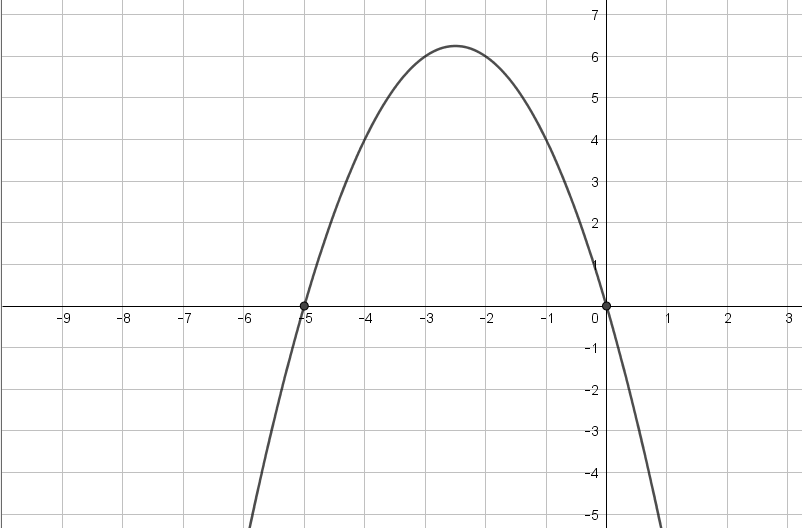
\includegraphics[width=2in]{GraphParabola1.png}
\end{frame}

\begin{frame}[t]{Intercepts}
Find the intercepts of the equation $4x + 5y = 40$.

\pause

Graph:

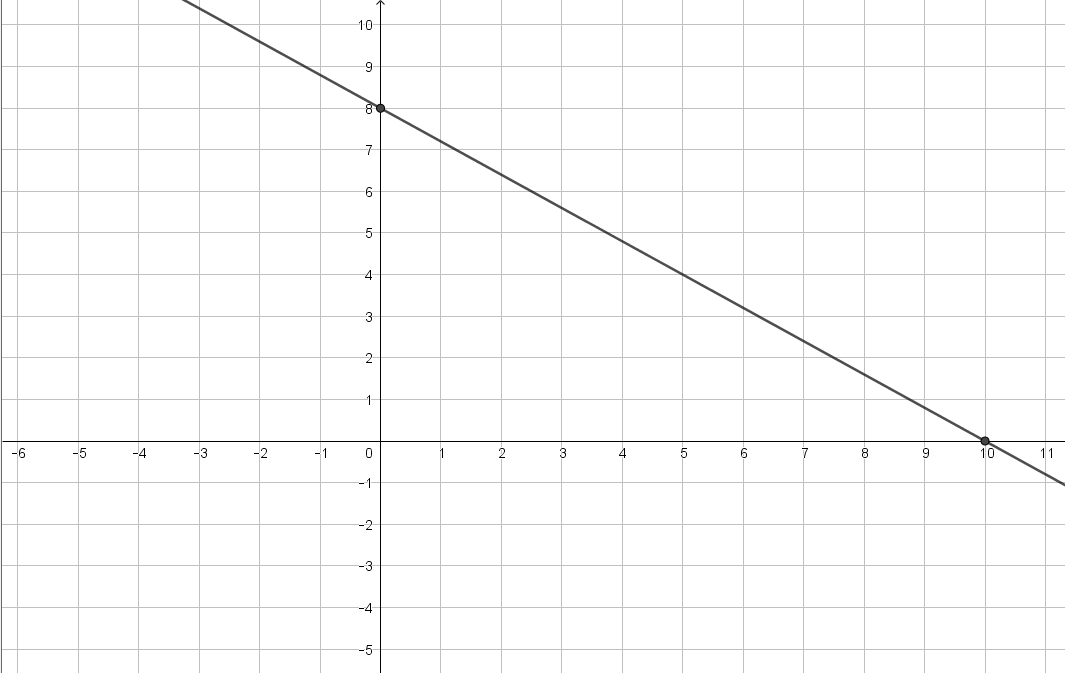
\includegraphics[width=2.5in]{GraphLine2.png}
\end{frame}

\begin{frame}[t]{Symmetry}
\begin{block}{Graphical Tests of Symmetry}
\begin{enumerate}[1)]
\item About the $x$-axis: whenever $(x,y)$ is on the graph, $(x,-y)$ is on the graph
\item About the $y$-axis: whenever $(x,y)$ is on the graph, $(-x,y)$ is on the graph
\item About the origin: whenever $(x,y)$ is on the graph, $(-x,-y)$ is on the graph
\end{enumerate}
\end{block}
\end{frame}

\begin{frame}[t]{Symmetry}
Graph each function in GeoGebra and check it for symmetry about the $x$ axis, about the $y$ axis, and about the origin.
\begin{enumerate}[(a)]
\item $y = x^2 - 1$
\item $x = 3y^4$
\item $x^2 + y^2 = 9$
\end{enumerate}

\pause

(a) Is symmetric about the $y$ axis only \\ \pause
(b) Is symmetric about the $x$ axis only \\ \pause
(c) Is symmetric about both axes and the origin
\end{frame}

\begin{frame}[t]{Symmetry}
\begin{block}{Algebraic Tests of Symmetry}
\begin{enumerate}[1)]
\item About the $x$ axis: replacing $y$ with $-y$ yields same equation
\item About the $y$ axis: replacing $x$ with $-x$ yields same equation
\item About the origin: replacing $y$ and $x$ with $-y$ and $-x$ yields same equation
\end{enumerate}
\end{block}
\end{frame}

\begin{frame}[t]{Symmetry}
Test the equation $x - y^2 = 1$ for symmetry about the $x$ axis, the $y$ axis, and the origin.

\pause \vfill

Test the equation $x^2 + y^2 = 9$ for symmetry about the $x$ axis, the $y$ axis, and the origin.

\end{frame}

\begin{frame}[t]{Linear Equations in One Variable}
\begin{block}{Definition}
A \textit{linear equation in one variable} is an equation that can be written in the form $ax + b = 0$ where $a,b\in\R$ and $a \neq 0$.
\end{block}

\pause

Example: Solve for $x$: $\dfrac{3x}{4} + \dfrac{x}{3} = 2$

\pause \vfill

Solve for $y$: $7y - 13 = 4y + 23$
\end{frame}

\begin{frame}[t]{Solving Linear Equations}
Solve for $x$: $\dfrac{3x}{x-4} = 5 + \dfrac{12}{x-4}$

\pause \vfill

Since $x = 4$ is not a solution to the original equation (plugging it in results in division by zero), we call $x = 4$ an extraneous solution to the equation.
\end{frame}

\begin{frame}[t]{An Application}
The number $y$ (in thousands) of male participants in high school lacrosse in the U.S. from 2008 through 2015 can be approximated by the linear model $$y = 3.66t + 91.4, \; \text{ } -2\leq t\leq 5$$ where $t$ represents the year, with $t=0$ corresponding to 2010. \begin{enumerate}[(a)]
\item Find and interpret the $y$-intercept.
\item Use the model to predict when there will be 128,000 participants.
\end{enumerate}
\end{frame}

\begin{frame}[t]{Next Steps}
\begin{itemize}
\item Complete Assignment \#2
\item Begin Module \#3
\begin{itemize}
\item Read 1.3 and 1.4
\item Watch Video Lesson \#5
\end{itemize}
\end{itemize}
\end{frame}

\end{document}